\section{Clinical Context} % (fold)
\label{sec:clinical_context}

This section describes our findings from the interview sessions. These findings form the basis of our use cases as well as some functional requirements. We will discuss both similarities and differences found in clinical practices as well as describing the patient monitoring solutions deployed today. Throughout this section we will refer to the three most important stakeholders, which is listed below:

\begin{itemize}

  \item[\textbf{Patients}] The patients themselves are the main source of physiological data. The patients are the ones in direct contact with the sensory equipment, and will act as the wearer of the WBANs. It is important to remember that these are people admitted to the hospital with a broad span of medical conditions. They might be in pain, unconscious, or mentally exhausted. One must take these considerations into the design and requirement specification.
  
  \item[\textbf{Practitioner}] We define health practitioners and clinicians are the medical staff that are responsible for care and treatment of patients, as well as operating their respective wards, departments or units. They are the ones that will install the sensors on the patient, and monitor the signal as they arrive at the central.

  \item[\textbf{Engineer}] Clinical engineer is defined as the medical and biomedical maintenance engineer responsible for installing and maintaining the technical equipment used for medical purposes at hospitals. Among other things, they are responsible for doing technical maintenance on the central heart monitoring system, which is as close as we come to an established way of monitoring vital signs wirelessly of multiple patients in hospitals today.

\end{itemize}

The rest of this chapter will be organized as follows: First we will discuss cardiac patients, the practice of patient monitoring and the intended use for our prototype. Then we will be taking a look at the existing solutions deployed at two Norwegian hospitals today, before ending this chapter with a detailed overview of different use cases.

\subsection{Intended use} % (fold)
\label{sub:intended_use}

The researcher from The Intervention Centre made it clear that we had to consider the intended use for our prototype. Monitoring ambulatory patients is merely an action following an intention, not the goal in itself. Therefore we must ask, for what patients are we developing this solution? What use-cases? What is the intended use?

Before we answer these questions, a little introduction to cardiac patients and patient monitoring in practice is needed. Most patients in a hospital today are not electronically monitored on a daily basis. There are however certain units in a hospital that monitor patients continuously. In the Intensive Care Unit (ICU) as well as the Postoperative Unit (PO) all patients are monitored (ECG, SpO$_2$ etc.) around the clock regardless of their diagnosis. The same accounts for Heart failure Units (HFU) and Intermediate Care Units (IMC) which are wards for patients with cardiac conditions and intravenous medications that require continuous cardiac monitoring and treatment. Depending on the hospital it may have one, two or all four units. All these units usually holds patients temporary before and after a surgical procedure or intervention - here meaning catheter based non-surgical procedures. When asking the cardiovascular surgeon about common heart disease diagnoses at these units, he said the following: 

\begin{quote} 
\textit{``Acute Coronary Syndrome (ACS) is a group of conditions related to a decreased blood flow in the arteries to the heart, also known as the coronary arteries, resulting a “myocardial ischemia”. This cause a shortage og oxygen and glucose needed for cellular metabolism and makes the heart muscle unable to contract properly and in worst case it will die. This is called a myocardial infarction, better known as a “heart attack”. These coronary artery diseases are the most common cause of death globally. Typically for all ACSs is that they are often diagnosed by ECG. Patient having an ACS needs a continuous monitoring before, during and after therapy, sometimes for days and sometimes even for weeks. Patients at the IMC, or those transferred to normal wards and to rehabilitation may still suffer from different consequences after a myocardial infarction like cardiac arrhythmias and even new cardiac ischemia.''}
\end{quote}
\noindent
This is the reason why patients at risk are fitted with a telemetry in order to be monitored. The clinician(s) at a monitoring central observes the heart rhythm and looks for signs of unusual elevations or interval variations in the QRST complex. See Table~\ref{tab:characteristicECGintervals}. Abnormalities above or below a given threshold often generate alarm triggering events. The thresholds comes with a default setting and is customizable per patient in the monitoring central. 

There is typically one such monitoring central at a given hospital. But where it is located varies. At the first hospital we visited, the central monitoring capability was located in a dedicated HFU. The second hospital didn't have a dedicated HFU, and the central monitoring station was located at the intensive care unit.s

Based on the observations above we define the intended use for this system as follows:

\begin{quote}
\textbf{Intended use:} To remotely monitor not critically ill patients at risk for complications regarding an acute coronary syndrome (susceptible for heart defects), located at an IMC or in another ward.
\end{quote}
\noindent
In other words, the intended use is on patients that would have been equipped with a telemetry device today. The existing systems are used for monitoring patients that are expected to experience, or are vulnerable to, heart defects either pre or post surgery, or during treatment. See table Table~\ref{tab:characteristicECGintervals} for a description of the most common irregularities and what identifies them. Because irregularities can happen at any time of the day and night, continuous monitoring is a fundamental requirement to the prototype.

% subsection intended_use (end)

\subsection{Existing Solutions} % (fold)
\label{sub:existing_solutions}

Interviews with medical engineers at both hospitals revealed that both had the Philips IntelliVue telemetry system installed. In both cases the network infrastructure and equipment was produced by Philips, but was delivered and maintained by different local partners. This section will describe the IntelliVue telemetry system from Philips, which as we found out, is deployed at several Norwegian hospitals today. The studying these systems were conducted in order to gain insight in the practice of wireless patient monitoring today, as well as giving us an indication of how prepared hospitals are for WBANs from a infrastructural point of view.

\subsubsection{System Architecture} % (fold)
\label{ssub:system_architecture}

The Philips IntelliVue telemetry system is a complete end-to-end system enabling both wired and wireless monitoring of ECG. For the medical practitioners the system is composed of two components: the TRx4841/51A wireless transceivers and the IntelliVue Information Centre. The TRx transceivers are devices for capturing ECG and SpO$_2$ on adult and pediatric patients, and are worn by the patients. Powered by two AA batteries they capture and stream a 3 or 5 lead ECG to a custom 802.11 type access point (AP) operating in the 2,4 GHz spectrum. These APs are installed in addition to, and independent of existing public or private WiFi access points. Because Philips provide all hardware in this closed system, the telemetry system does not have to confine to the interoperability requirements it would needed if the system were to allow for proprietary sensors and measuring devices. The wireless interface is based on the 802.11 specification, and the system offer a ``Smart Hopping'' technology in order to reduce collisions on the already crowded 2,4 GHz network band. This is made possible by synchronizing all access points through a dedicated sync unit. Another noteworthy network feature is the ``make before break'' method that improves the roaming abilities. The TRx transceivers will look for new, stronger access points when they detect a decay in signal strength with the current AP. The system will make sure to connect transceivers to the new (stronger) AP before breaking with the previous one, enabling a more reliable handoff between access points. The network coverage at the second hospital were almost 100\%, while the first, larger hospital offered 100\% network coverage in one of it's buildings.

\begin{figure}[H]
  \centering
  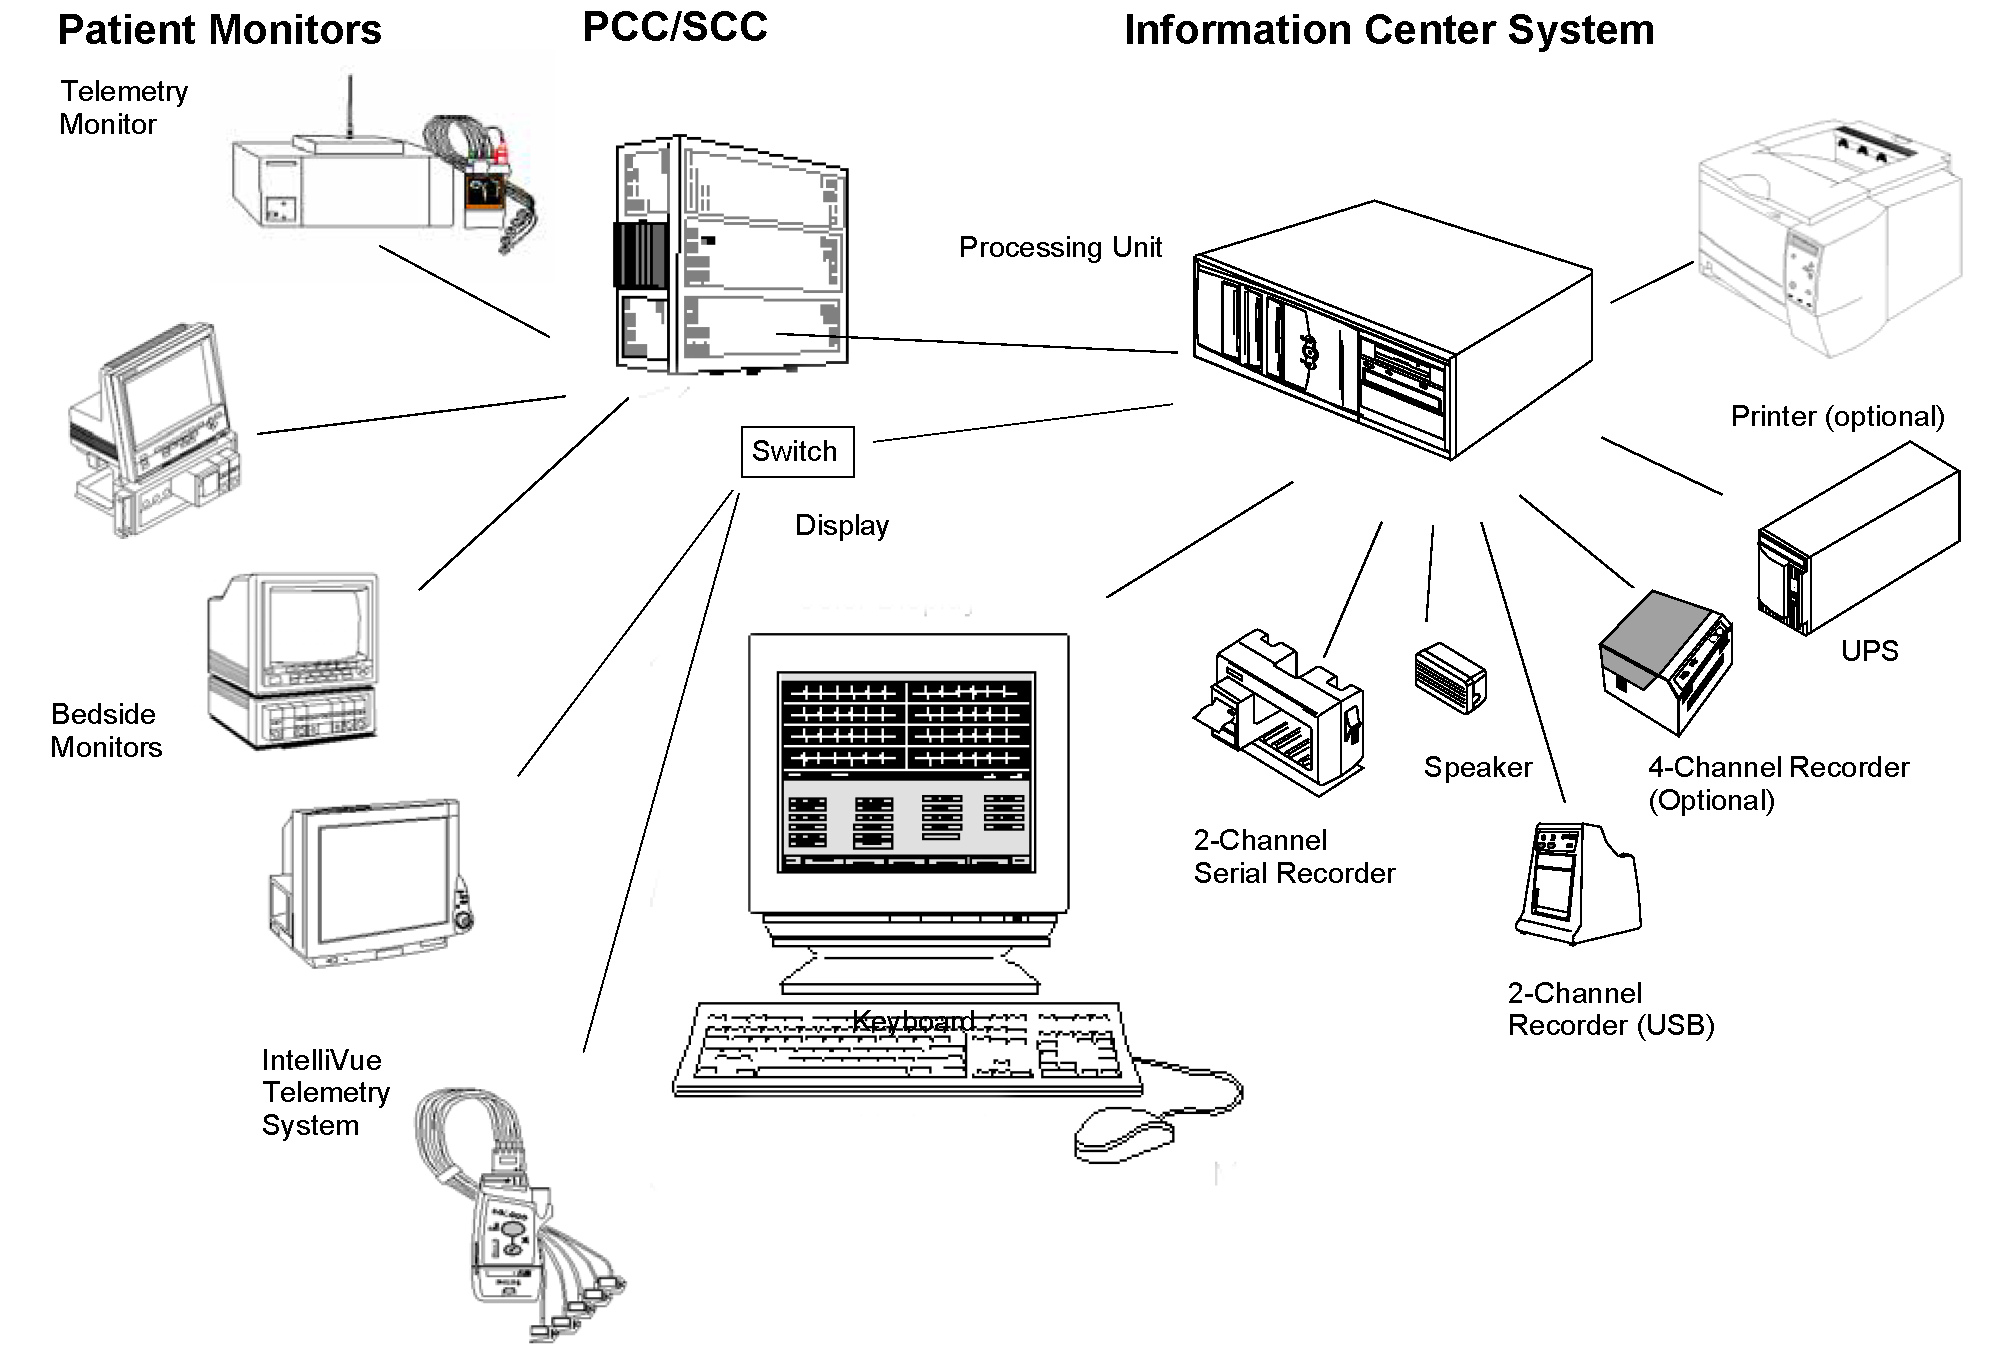
\includegraphics[scale=.7]{img/figures/philipsintellivue.png}
  \caption{IntelliVue Monitoring System Components~\cite{IntelliVue:telemetry}}
  \label{fig:intellivue_telemetry_architecture}
\end{figure}


As mentioned, this being a end-to-end system the IntelliVue patient monitoring suite includes everything from transceivers, bedside monitors, access points, synchronization units, gateways, network switches, uninterruptible power supplies (UPS), processing units and databases in addition to the optional printer Figure~\ref{fig:intellivue_telemetry_architecture}.

\begin{figure}[H]
  \centering
  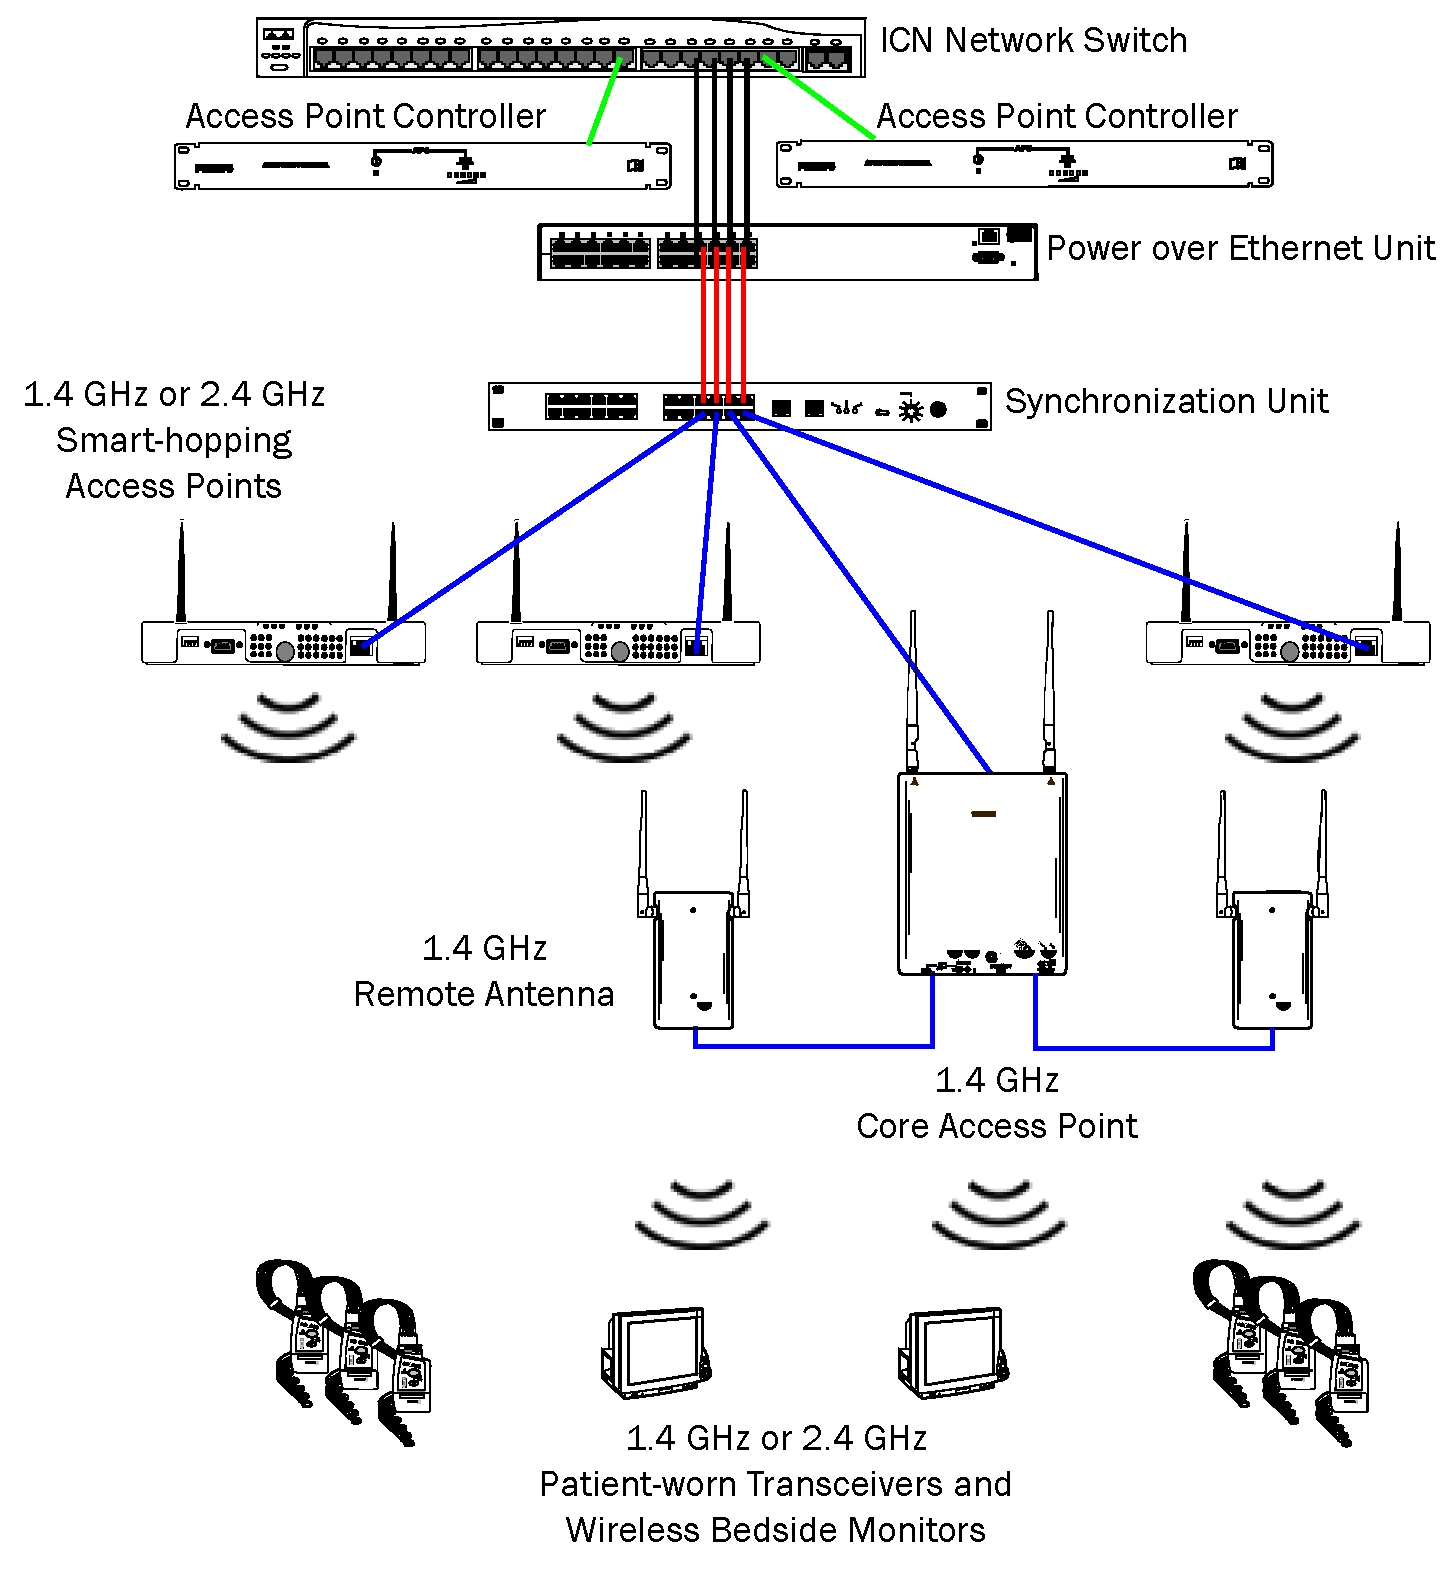
\includegraphics[scale=.6]{img/figures/philipsintellivue2.png}
  \caption{IntelliVue Network Topology~\cite{IntelliVue:telemetry}}
  \label{fig:intellivue_telemetry_architecture2}
\end{figure}

Offering every piece in this architecture enables Philips and its local distributers and providers to guarantee good QoS metrics which is essential for wireless patient monitoring applications. However, installing a complete system like this comes with a substantial economic cost, and ties you down to just one provider for an extended period of time. The IntelliVue Telemetry system at the first hospital was installed in 2009, and is expected to have a lifespan of at least 10 years. This reduces the flexibility and ability to adapt new solutions. On the upside, an all-in-one solution like can easier guarantee QoS as well as offering better support and maintenance. It's easy to think that this also might reduce the need for interoperability - because Philips controls the whole stack. Having studied the solution being used in practice, we would argue this is false. An example of this can be found in the installation of the CorPulse ECG device from Alere \cite{alere}. This is a device installed in emergency vehicles enabling a short, pre-hospital ECG to be sent over 3G network with a SIM card. This is often critical information that enable the medical staff to make informed decisions before the patient arrives at the hospital. Because this is a different system from a different provider, the hospitals we visited had installed a standalone computer next to the central monitoring information center system from Philips. This standalone computer display the pre-hospital ECG from the Alere device. Although coming from a different source, the users we talked to experienced this as ``remote ECG'', just as the they experienced the central telemetry solution next to it as ``remote ECG''. This is suboptimal not only in technical terms and with regards to maintenance, but also from a user experience point of view. The lack of integrations creates yet another technical dependency in the everyday life of medical practitioners. A workaround for dealing with separate systems is sharing login credentials, which render the security measure completely useless. We observed this at one of the hospitals. Based on these observations, we believe interoperable devices and services will be crucial for the success of a ubiquitous, sensor-based health care.

% subsubsection system_architecture (end)

\subsubsection{The Transceivers} % (fold)
\label{ssub:the_transceivers}

\begin{wrapfigure}{r}{0.3\textwidth}
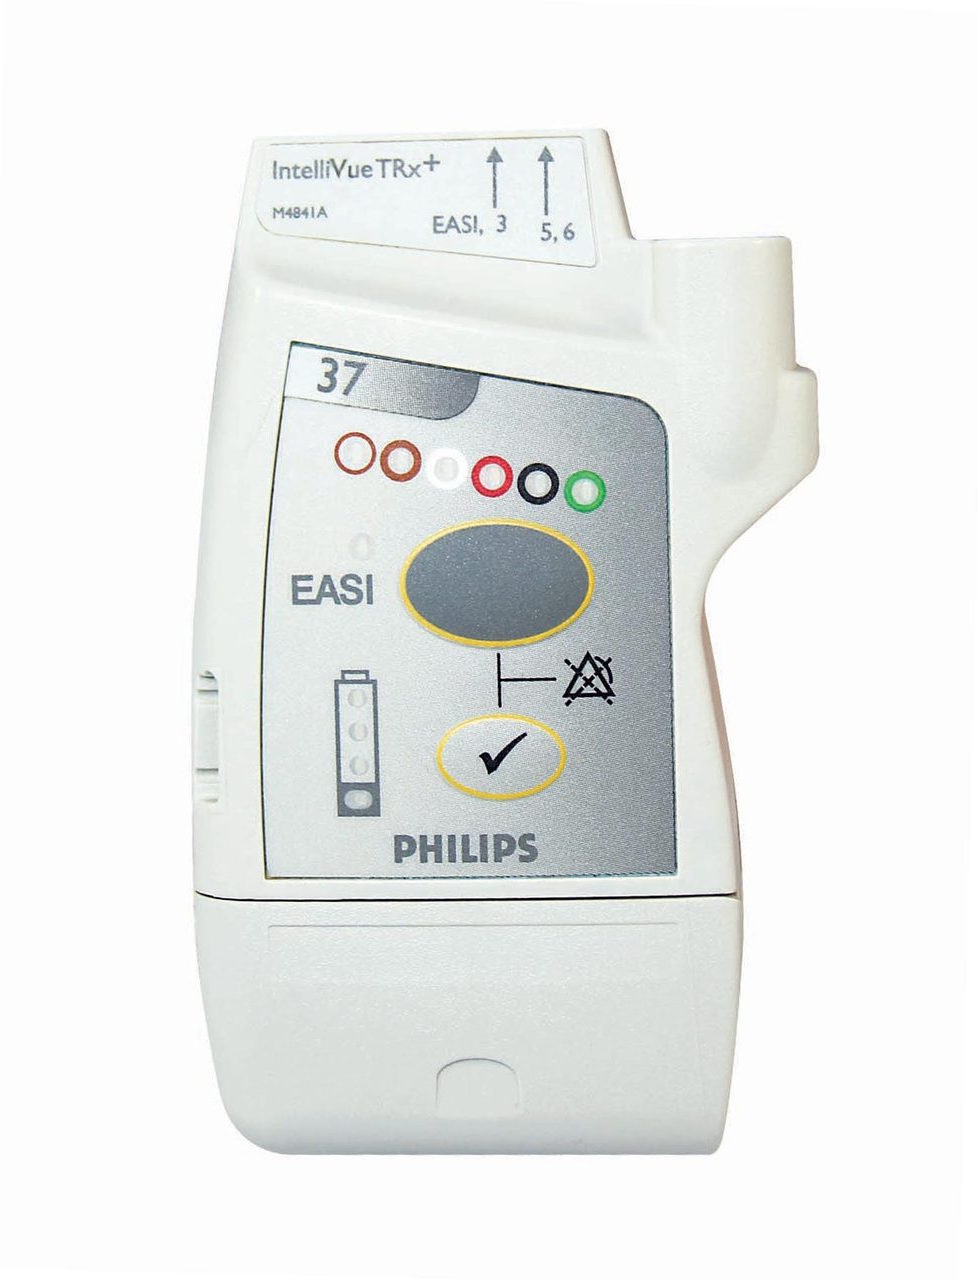
\includegraphics[width=1\linewidth]{img/trx.jpg} 
\caption{TRx transceiver from Philips}
\label{fig:subim1}
\end{wrapfigure}

The TRx transceivers are small and lightweight with a limited user interface consisting of a couple of lights and a audible alarm. In practice we were told they have a battery lifetime a little over 24 hours, which fits well with the specifications found in the user manual (up to 48 hours). As we'll see in Section~\ref{ssub:maximum_throughput}, the average throughput is tied to sampling rate. In order to establish a standard for what throughput wireless ECG must support we reviewed both literature and the user manuals for the IntelliVue Telemetry system. As the numbers used in literature varies a lot, we searched the user manuals for this information. However, we were unable to find any information about neither the sampling rate nor average throughput the transceivers delivered. Both Philips and the local providers of the system were consulted, but no one could give us a clear answer. When this failed, attempts were made to find the information based on network traffic, but we never got hold of the telemetry network administrator.

In terms resolution, Philips Medical Systems have developed the ``EASI'' lead system with the ability to estimate a 12 lead ECG. This is in line with the results from \cite{Wehr:2006ht} Wehr et. al. which showed that the 5-electrode EASI was equivalent to a 12-lead ECG for the diagnosis of myocardial ischemia. Although the transceivers provide ambulatory and bedside patient monitoring, there's a catch with increasing the mobility: Usually when doing a detailed 12-lead ECG, medical practitioners place the 4 extremity electrodes at the wrists and ankles. In a 5-lead telemetry these electrodes are often moved to shoulders, hips and chest in order to increase mobility. However, because of the large muscle mass located in these areas, the recorded ECG signal is prone to more muscle noise. We observed this ourself while studying a distorted 5-lead telemetry reading at one of the hospitals. We were told this probably was a result of the patient moving. Accurate, unobtrusive and noise resilient sensors like the ones in \cite{ChulsungPark:2006tf, Anonymous:FtVb5yQr} will be an absolute necessity in persuasive patient monitoring. 

If there should be extended periods of noise or the clinicians are suspicious with the readings on the screen, they have the ability to do an independent ECG. Both ICU and the unit with the remote patients had several standalone 12-lead ECG units that could be connected to the patient on request. We observed how a patient could be connected to the standalone ECG device with 10 electrodes in order to get the full 12-lead resolution. This device was mobile (on wheels) and had the form factor of a small laptop computer. It was standalone in the sense that it's only output was a printed time interval of 6 seconds from the examination as shown in Figure~\ref{fig:pappa_ecg} from a built in printer.
We also visited two other medical units at the same hospital that did some ECG monitoring. Both of which used a 3-lead setup connected directly to a bedside monitor. This stands to show that at the second hospital, 3 and 5-lead setups are most used in continuous monitoring. The full 12-lead was only used in short examinations on demand. This practice was also confirmed at the Clinic of Cardiology at the first hospital.

\begin{figure}[H]
  \centering
  \includegraphics[scale=.6]{img/figures/ecgplot.png}
  \caption{Annotated ECG plot of lead V1-V6. See Appendix~\ref{sec:ecg_plot} for all 12-leads.}
  \label{fig:pappa_ecg}
\end{figure}


% subsubsection the_transceivers (end)

\subsubsection{The Information Centre} % (fold)
\label{ssub:the_information_centre}

The Philips IntelliVue Information Center constitute the the central monitoring post. Here clinicians has the ability to view multiple real-time patient leads at once, see detailed view on a given patient, and adjust alarms and thresholds. The IntelliVue Telemetry System supports up to 128 2,4Ghz transceivers.

% TODO Kanskje noe om lagring? I så fall måtte det bli for å snakke om 

% an provide a web view for accessing the patient data from outside the monitoring central. According to the service manuals they claim that the information displayed in the web view should be near-real time with little delay, but recommend users to always use the bedside monitor or the information center for real-time monitoring.

To this project, the most interesting aspects of the monitoring central was the end-to-end latency between the electrode on the patient to the central. We were unable to find an accurate metric for the end-to-end latency in IntelliVue's documentation. Information on transmission delay is also scarce in the literature we reviewed. Within the field of WBAN very few address this issue, and and we had to look into Telemedicine in order to find any suggestions to end-to-end latency at all. Through clinical trails, Alesanco and Garcia suggest 3-4 seconds as the maximum acceptable delay for a reliable real-time ECG transmission \cite{Alesanco:2010kc}. Their research however is concerned with telemedicine over 2G/3G networks, where the intended use and QoS are different. 
Because Philips have full control over the whole infrastructure and the distances at a hospital are relatively small, it is reasonable to assume the delay from the measurement to the information center is less than 2 seconds. An alternative approach to getting information about acceptable transmission delay would be to measure the actual network traffic in the systems deployed today. But as mentioned, we were unsuccessful in getting in touch with the network administrator at either hospitals.

As Alesanco and Garcia's requirement was the only exact metric we could relate to, we chose to use this as our baseline for network delay.

% subsubsection the_information_centre (end)

\subsection{Use Cases} % (fold)
\label{ssub:use_cases}

% TODO Skriv om hvilke krav som stilles i hver use case. ta en titt på quality attributes-skjemaet

Having established the intended use, we will use this section to describe different use cases. We believe this has to be included in order to get an understanding of the context the solution have to support. Keep in mind that these use cases only assess some parts of the system, and cover more practical features rather than technical.
\\
\newline
\noindent
\textbf{Patient}
\begin{enumerate}

  \item[\textsc{U1}:]\textbf{Stationary:} This use case will describe the situation where a patients monitored while lying in bed. Here both gateway and sensor would be stationary.
  
  A patient is being monitored wirelessly while lying in bed.
  

  \item[\textsc{U2}:]\textbf{Partly ambulatory:} Here patients are monitored while walking around their bed. This means the patient is ambulatory while the gateway is stationary.

  \item[\textsc{U3}:]\textbf{Ambulatory:} This use case describe the situation where patients are monitored while walking around the room or ward, with the personal gateway in their pocket. This means the patient is fully ambulatory.

\end{enumerate}

\noindent
\textbf{Medical Professional}
\begin{enumerate}

  \item[\textsc{U4}:] Setting up the patients personal gateway
  \item[\textsc{U5}:] Monitor a patients ECG on a separate device

\end{enumerate}


\newline

\begin{table}[H]
\renewcommand{\arraystretch}{1.2}
\captionof{table}{Use case: Stationary}
\begin{tabular}{|p{4cm}|p{9cm}|}
\hline
ID & U1 \\ \hline
Name & Stationary \\ \hline
Goal & \begin{tabular}[c]{@{}l@{}}
Store ECG data using a stationary sensor and a\\ stationary gateway.
\end{tabular} \\ \hline
Actors &  Patient\\ \hline
Start requirements & \begin{tabular}[c]{@{}l@{}}
1. Mobile gateway is connected to the sensor\\
2. Mobile gateway is connected to the local WiFi.
\end{tabular} \\ \hline
End requirements & \begin{tabular}[c]{@{}l@{}}
Patient ECG stream is transmitted to the monitoring\\ station and the data is stored.
\end{tabular} \\ \hline
Main flow & \begin{tabular}[c]{@{}l@{}}
The gateway is activated and data gets routed\\ from sensor to network.
\end{tabular} \\ \hline
Alternative flow & \begin{tabular}[c]{@{}l@{}}
None
\end{tabular} \\ \hline
Parent use case & None \\ \hline
Child use case & U2 \\ \hline
\end{tabular}
\end{table}

\begin{table}[H]
\renewcommand{\arraystretch}{1.2}
\captionof{table}{Use case: Partly Ambulatory}
\begin{tabular}{|p{4cm}|p{9cm}|}
\hline
ID & U2 \\ \hline
Name & Partly Ambulatory \\ \hline
Goal & \begin{tabular}[c]{@{}l@{}}
Store ECG data while having a moving\\ sensor and a stationary gateway.
\end{tabular} \\ \hline
Actors &  Patient\\ \hline
Start requirements & \begin{tabular}[c]{@{}l@{}}
1. Mobile gateway is connected to the sensor\\
2. Mobile gateway is connected to the local WiFi.\\
3. The gateway is activated and data gets routed\\ from sensor to network.
\end{tabular} \\ \hline
End requirements & \begin{tabular}[c]{@{}l@{}}
Patens are able to move freely around their beds\\ while the gateway is stationary on the nightstand.
\end{tabular} \\ \hline
Main flow & \begin{tabular}[c]{@{}l@{}}
Patients are able to get out of bed and move walk\\ around undisturbed.
\end{tabular} \\ \hline
Alternative flow & \begin{tabular}[c]{@{}l@{}}
None
\end{tabular} \\ \hline
Parent use case & U1 \\ \hline
Child use case & U2 \\ \hline
\end{tabular}
\end{table}

\begin{table}[H]
\renewcommand{\arraystretch}{1.2}
\captionof{table}{Use case: Ambulatory}
\begin{tabular}{|p{4cm}|p{9cm}|}
\hline
ID & U3 \\ \hline
Name & Ambulatory \\ \hline
Goal & \begin{tabular}[c]{@{}l@{}}
Store ECG data having a both a moving sensor\\ and a moving gateway.
\end{tabular} \\ \hline
Actors &  Patient\\ \hline
Start requirements & \begin{tabular}[c]{@{}l@{}}
1. Mobile gateway is connected to the sensor\\
2. Mobile gateway is connected to the local WiFi.\\
3. The gateway is activated and data gets routed\\ from sensor to network.
\end{tabular} \\ \hline
End requirements & \begin{tabular}[c]{@{}l@{}}
1. Patens can move freely outside their room.\\
2. The gateway automatically connects to new\\ access points.
\end{tabular} \\ \hline
Main flow & \begin{tabular}[c]{@{}l@{}}
Patients pick up the mobile gateway and walks out\\ of the room.
\end{tabular} \\ \hline
Alternative flow & \begin{tabular}[c]{@{}l@{}}
None
\end{tabular} \\ \hline
Parent use case & U2 \\ \hline
Child use case & None \\ \hline
\end{tabular}
\end{table}


% TODO Insert figures
% \begin{figure}[H]
% \centering
% 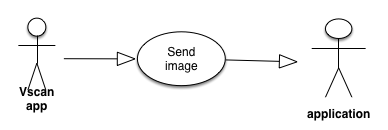
\includegraphics[scale=0.8]{img/usecase/receive.png}
% \caption{Receive images from Vscan}
% \label{fig:receive_image_uc}
% \end{figure}

\begin{table}[H]
\renewcommand{\arraystretch}{1.2}
\captionof{table}{Use case: Set up gateway}
\begin{tabular}{|p{4cm}|p{9cm}|}
\hline
ID & U4 \\ \hline
Name & Set up gateway \\ \hline
Goal & \begin{tabular}[c]{@{}l@{}}
The gateway is configured and ready to proxy\\sensor node data to endpoint
\end{tabular} \\ \hline
Actors &  Clinician\\ \hline
Start requirements & \begin{tabular}[c]{@{}l@{}}
1. Sensor node and gateway have sufficient battery.\\
2. The clinician is authenticated and authorized\\
to configure the gateway application.\\
3. Monitoring server is running.
\end{tabular} \\ \hline
End requirements & \begin{tabular}[c]{@{}l@{}}
The gateway is ready to stream data from the sensor\\
node to the endpoint.
\end{tabular} \\ \hline
Main flow & \begin{tabular}[c]{@{}l@{}}
1. The clinician opens the application and click ``new''.\\
2. The clinician click scan for sensor and select\\
the correct sensor.\\
3. The clinician selects an endpoint from the list.\\
4. Clicks ``activate'' which test and activates the\\
gateway routing.
\end{tabular} \\ \hline
Alternative flow & \begin{tabular}[c]{@{}l@{}}
The gateway is not able to connect to either sensor\\
or endpoint. Error message is shown.
\end{tabular} \\ \hline
Parent use case & None \\ \hline
Child use case & U1,U2,U3 \\ \hline
\end{tabular}
\end{table}

\begin{table}[H]
\renewcommand{\arraystretch}{1.2}
\captionof{table}{Use case: Monitor ECG}
\begin{tabular}{|p{4cm}|p{9cm}|}
\hline
ID & U5 \\ \hline
Name & Monitor ECG\\ \hline
Goal & \begin{tabular}[c]{@{}l@{}}
The clinician is able to monitor a ECG plot\\
on a separate device.
\end{tabular} \\ \hline
Actors &  Clinician\\ \hline
Start requirements & \begin{tabular}[c]{@{}l@{}}
The clinician is authorized to monitor ECG.\\
\end{tabular} \\ \hline
End requirements & \begin{tabular}[c]{@{}l@{}}
The ECG stream is available at the clinicians\\
device
\end{tabular} \\ \hline
Main flow & \begin{tabular}[c]{@{}l@{}}
1. A clinician navigates to the correct URL\\
on a web enabled device.\\
2. The clinician selects the correct patient\\
and sees a live ECG plot in her web browser.
\end{tabular} \\ \hline
Alternative flow & \begin{tabular}[c]{@{}l@{}}
The clinician is not authorized and do not\\
get access to the ECG stream.
\end{tabular} \\ \hline
Parent use case & U4 and U1 or U2 or U3.\\ \hline
Child use case & None\\ \hline
\end{tabular}
\end{table}

% section clinical_context (end)